\documentclass[a4paper,11pt]{article}
\usepackage[frenchb]{babel}
\usepackage[T1]{fontenc}
\usepackage[utf8]{inputenc}
\usepackage{lmodern}
\usepackage{microtype}

\usepackage{array,multirow,makecell}
\setcellgapes{1pt}
\makegapedcells
\usepackage{caption}
\usepackage{adjustbox}

\usepackage{amsmath,amssymb,bm,upgreek,stmaryrd,mathrsfs,systeme}

\usepackage{graphicx}

\usepackage{geometry}
\geometry{hmargin=3cm,vmargin=2cm}

\usepackage{hyperref}

\title{Premier modèle de la Terre comme système énergétique}

\begin{document}
\maketitle

\section{Description du modèle}

Pour tester le modèle, vous pouvez ouvrir le fichier Python "Modele\_1.py" pour faire la simulation. \\

On part des données suivantes :

\begin{enumerate}

\item[•] Puissance surfacique du Soleil reçu par la Terre : $P_S = 1300 ~ W \cdot m^{-2}$
\item[•] Rayon de la Terre : $R_T$ = 6371 km
\item[•] Constante de Stefan-Boltzmann : $\sigma = 5,67 \cdot 10^{-8} ~ W \cdot m^{-2} \cdot K^4$ \\

\end{enumerate}

Pour commencer, la puissance que reçoit la Terre correspond au produit de la puissance surfacique et de la surface de la Terre en considérant que la surface de la Terre est un disque pour connaître la puissance réelle reçue sur l'ensemble de sa surface. En notant $P_S$ la puissance surfacique du Soleil à la distance Terre-Soleil du Soleil, $P_{S/T}$ la puissance reçue par la Terre, S la surface du maître-couple (voir Table 1 dans Annexes) de la Terre et $R_T$ le rayon de la Terre, on a :

\[ P_{S/T} = P_S \cdot S = P_S \cdot \pi R_T^2  \]

Ensuite, en considérant que l'albédo moyen de la Terre est $A = 0.3$, ce qui est possible de justifier (cliquez \href{../m/fichier}{ici}), on obtient que la puissance réfléchie $P_r$ par la surface terrestre est :

\[ P_r = A \cdot P_{S/T} \]

En utilisant la loi de Stefan-Boltzmann, on connaît la puissance émise par la Terre $P_e$ :

\[ P_e = \sigma T^4 \cdot 4 \pi R^2 \]

Dans ce modèle, nous négligeons les effets internes de la Terre, ce qui implique que celle-ci n'émet de puissance que par ce qu'elle reçoit du Soleil, soit la puissance absorbée modélisée par la loi de Stefan-Boltzmann. On considère alors que la puissance reçue par la Terre $P_{S/T}$ est égale à la somme de la puissance réfléchie $P_r$ et de la puissance émise $P_e$ :

\[ P_{S/T} = P_r + P_e \]

Finalement, en remplaçant par les expressions explicitées précédemment et en isolant la température de la Terre $T$, on obtient :

\[ T = \left(\dfrac{(1 - A) \cdot P_S}{4\sigma}\right)^{1/4} \]

Dans ce modèle, la température est constante et  :

\[ T = -18,57 ^{\circ} C \]


\begin{adjustbox}{center}
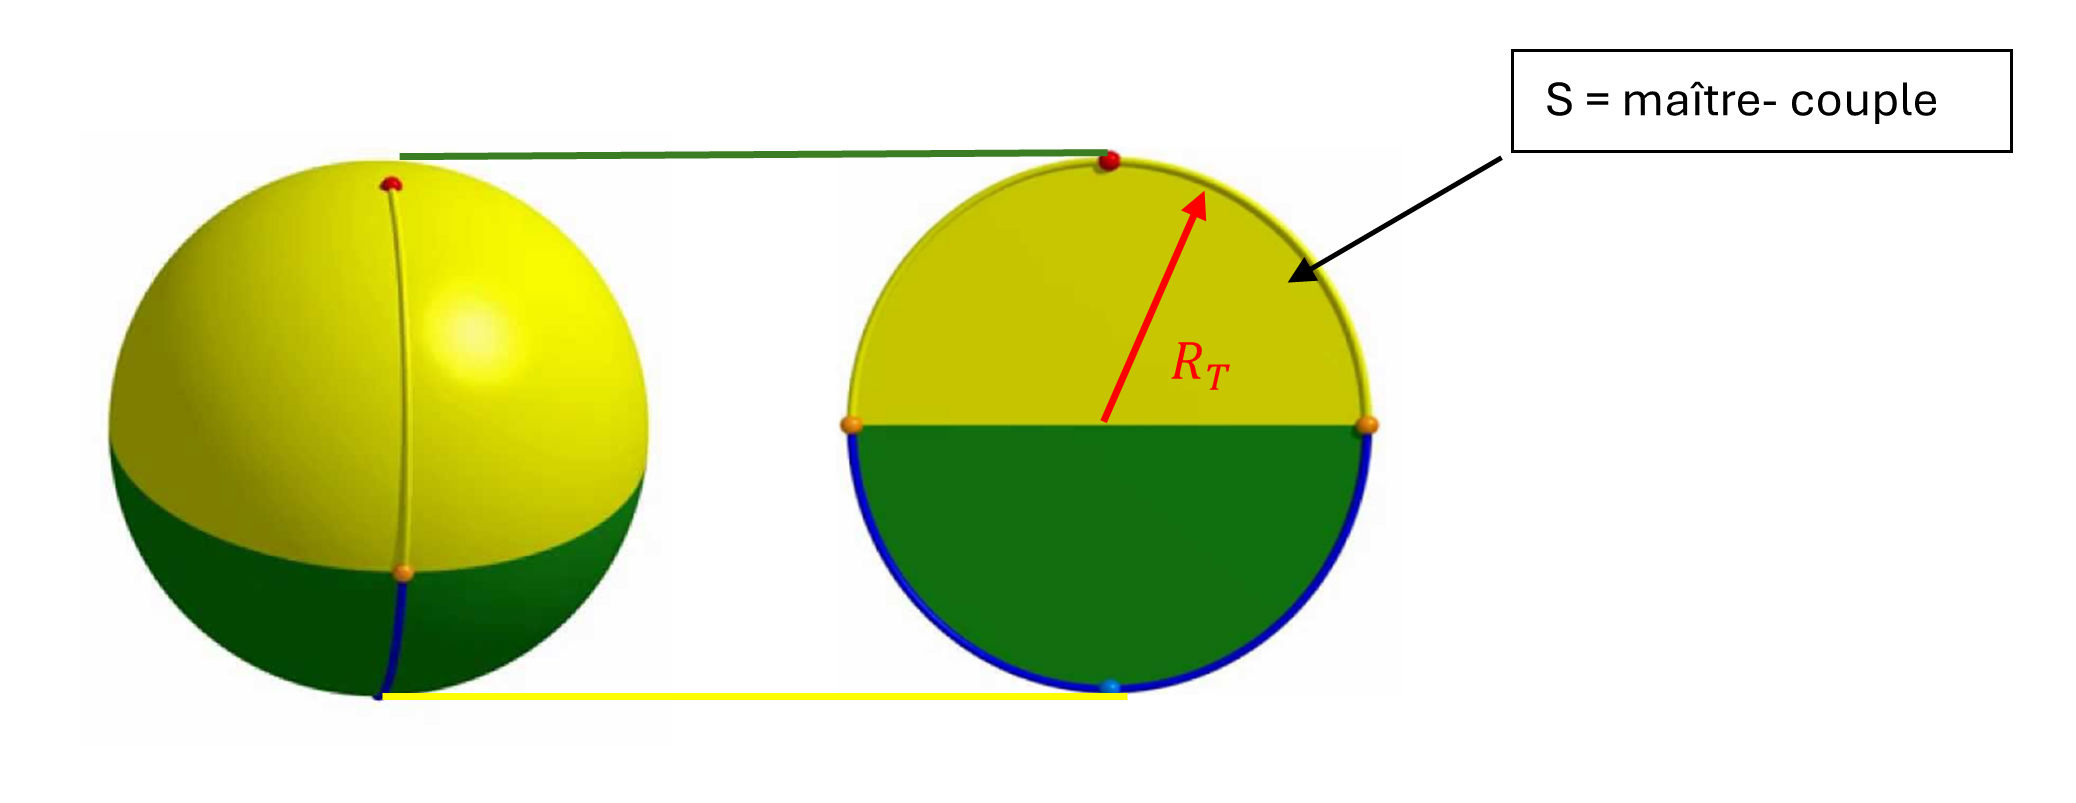
\includegraphics[scale=0.9]{Schema_maitre_couple}
\end{adjustbox}
\captionof{table}{Surface considérée (maître-couple) \\} 







\end{document}